% Template:     Informe LaTeX
% Documento:    Archivo de ejemplo
% Versión:      8.1.7 (24/07/2022)
% Codificación: UTF-8
%
% Autor: Pablo Pizarro R.
%        pablo@ppizarror.com
%
% Manual template: [https://latex.ppizarror.com/informe]
% Licencia MIT:    [https://opensource.org/licenses/MIT]

\section{Introducción}

Amazon.com,  es una empresa estadounidense de comercio electrónico y computación en la nube, fue fundada en julio de 1994. Es conocida por la tienda más grande del mundo tiene; libros, piezas de repuesto para automóviles, juguetes para niños, productos electrónicos, etc. También es conocida por fabricar artículos de consumo. electrónica: Amazon Kindle, Amazon Alexa, Echo y muchos más. Amazon también permitió que los autores y editores publicaran y pusieran a disposición sus libros en Kindle Store, con el brazo de publicación "Amazon Publishing". \scite{jopson2011amazon}

\begin{figure}[h]
	\centering
	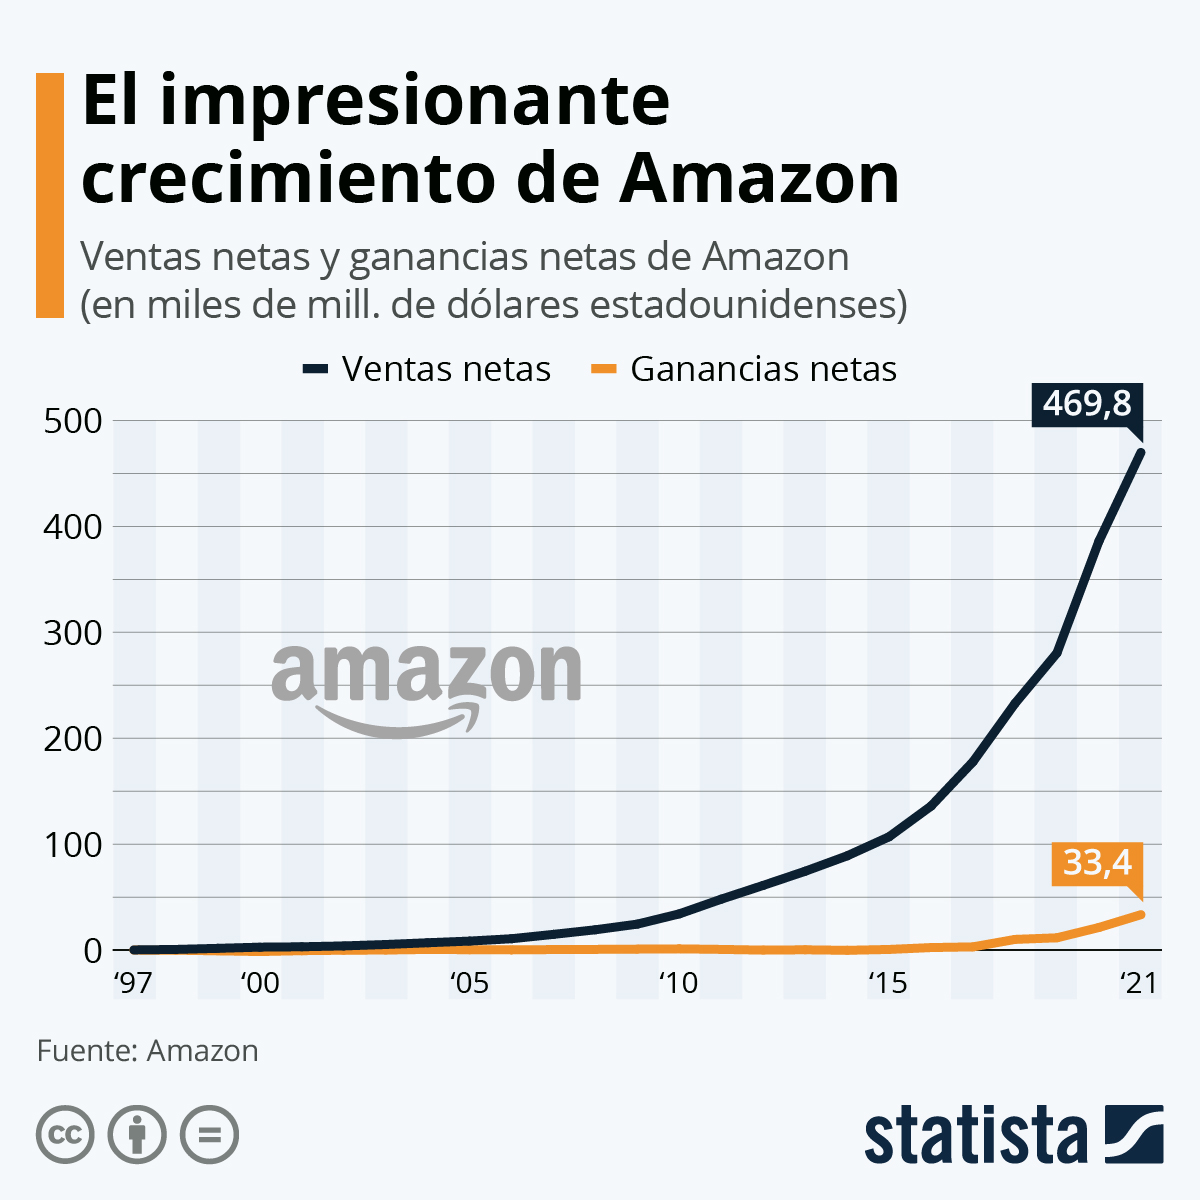
\includegraphics[scale=.2] {img/crecimiento_amazon}
	\caption{Crecimiento}
	\label{fig:1}	
\end{figure}

Amazon es el quinto sitio web más visitado a nivel mundial, con un total de 3,000 millones de visitas a septiembre de 2021, según datos de Semrush. El portal de comercio electrónico también registró 0.7 mil millones de visitantes únicos. \scite{semrush}

\subsection{Procesamiento y almacenamiento}
El sistema se evalúa en el catálogo de productos de Amazon, un gran conjunto de datos que comprende alrededor de 9 millones de productos, 144 millones de reseñas y una gran cantidad de metadatos \scite{singh2019analysis}

\textbf{¿Cuál es su necesidad?}


El sistema se evalúa en el catálogo de productos de Amazon, un gran conjunto de datos que comprende alrededor de 9 millones de productos, 144 millones de reseñas y una gran cantidad de metadatos \scite{singh2019analysis}. Estas reseñas dan confianza a los futuros compradores y condicionan la compra   o no del producto\scite{reseniaAmazon}.



\subsection{Amazon EMR Architecture \& Working}
Amazon mezcla y combina arquitecturas para satisfacer sus diversas necesidades comerciales. Amazon EMR Model analiza el mapa y reduce el big data. Amazon Elastic MapReduce proporciona usos sistemáticos y sencillos de la plataforma de análisis dentro del poderoso marco Hadoop que utilizan en gran medida algunas grandes empresas. El funcionamiento de Amazon EMR se basa en la arquitectura maestro/esclavo, mientras que el trabajo de Amazon EMR se basa en la arquitectura maestro/esclavo, mientras que los nodos maestros son parte del grupo de instancias de MapReduce y los nodos esclavos aún ejecutan HDFS y se convierten en más nodos principales. Las arquitecturas se ejecutan en la siguiente secuencia:
\begin{itemize}
	\item Amazon EMR envía una solicitud para iniciar un clúster.
	\item Amazon EMR crea el clúster de Hadoop con un nodo principal agregado a la instancia principal y un nodo central agregado al grupo principal.
	\item Un solo nodo maestro y muchos otros nodos esclavos procesan las tareas en el clúster.
\end{itemize}



“Amazon utiliza Amazon Elastic MapReduce (Amazon EMR) para sus procesos comerciales de comercio electrónico y en el análisis de una gran cantidad de datos distribuidos, administrados por el marco Hadoop, es rápido y rentable, adecuado para compras bajo demanda. Amazon EMR funciona en varios clústeres y los servidores se ejecutan en la arquitectura de nube distribuida de Amazon y administra big data, incluidos archivos de registro, indexación web, simulación científica, extracción de datos, almacenamiento de datos, inteligencia artificial y análisis de contabilidad seguros y confiables” \scite{zakir2015big}

\begin{figure}[h]
	\centering
	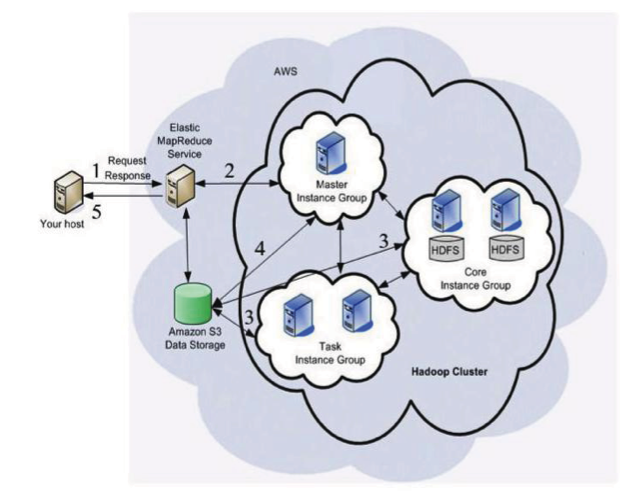
\includegraphics[scale=.4] {img/A-EMR-Arch}
	\caption{Amazon EMR Architecture}
	\label{fig:2}	
\end{figure}

AMAZON HADOOP: Hadoop es un concepto de marco de código abierto que admite la técnica de procesamiento de datos en un controlador de clúster múltiple de Amazon que utiliza una arquitectura maestra y esclava en muchos servidores. Amazon utiliza Amazon MapReduce para el procesamiento de grandes datos y para el almacenamiento de datos utiliza HDFS \scite{zakir2015big}
\begin{figure}[h]
	\centering
	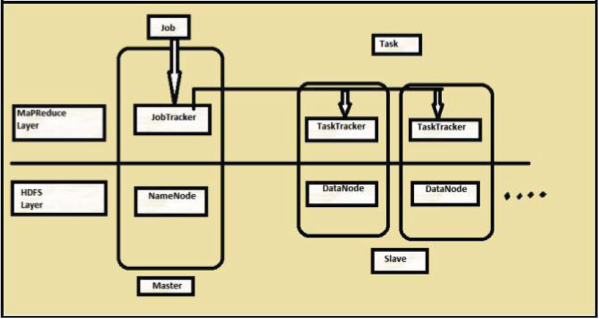
\includegraphics[scale=.4] {img/hadoop-w}
	\caption{Hadoop working, Fuente: \scite{verma2018beyond}}
	\label{fig:3}	
\end{figure}


Amazon desarrolló sofisticados motores de recomendación que entregan más del 35\% de todas las ventas soportadas en Big Data, sistemas automatizados de servicio al cliente para garantizar una satisfacción superior del cliente y sistemas de precios dinámicos que ajustan los precios en comparación con los sitios de la competencia \scite{agarwal2014big}

\subsection{El proceso de Big Data de Amazon}

El proceso de big data \scite{chen2017application} de Amazon se divide en tres etapas: recopilación y aplicación artificial, sistema de recomendación principal, que fue más complejo para construir el sistema de datos, como la Figura \ref{fig:4}. y sistema de información logística, nuevo sistema de recomendación de datos y sistema de gestión logística, como Figura \ref{fig:5}.

\begin{figure}[h]
	\centering
	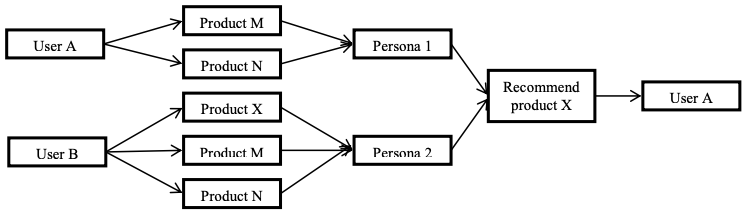
\includegraphics[scale=.5] {img/recomendation-system}
	\caption{Sistema de recomendación por asociación de usuario: \scite{singh2019analysis}}
	\label{fig:4}	
\end{figure}

\begin{figure}[h]
	\centering
	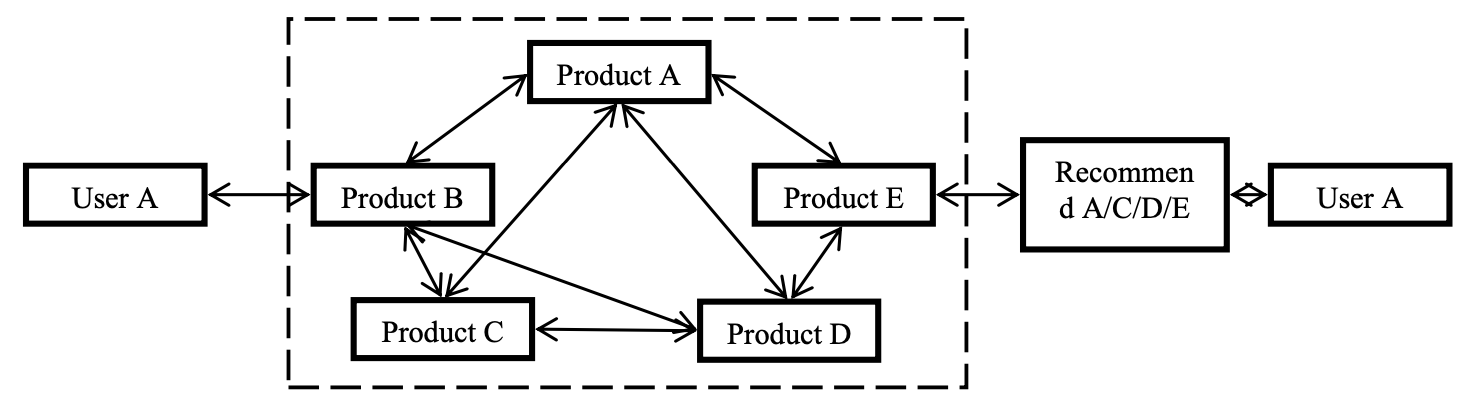
\includegraphics[scale=.3] {img/asocacion_productos}
	\caption{Sistema de recomendación por asociación de productos, Fuente: \scite{singh2019analysis}}
	\label{fig:5}	
\end{figure}


\subsection{Cuál es su necesidad}

Para empresas como Amazon y muchas otras, la cantidad de datos recopilados de forma regular es enorme. Para administrar y procesar grandes cantidades de datos, Amazon aprovecha la tecnología Big Data para hacer el trabajo por ellos. Esencialmente, Big Data es la recopilación a gran escala de información utilizada para análisis e información. Big Data recopila cada clic, me gusta, comentario y transacción. Es lo que permitió construir toda una industria sobre almacenes masivos de información\scite{bigDataAmazon}.

% ------------------------------------------------------------------------------
% NUEVA SECCIÓN
% ------------------------------------------------------------------------------

\subsection{Cómo lo utiliza}
Entonces, Amazon tiene los datos, pero ¿cómo los obtuvieron? La razón por la que son líderes en almacenamiento, procesamiento e implementación de datos es porque tienen algunos de los programas de recopilación de datos más efectivos. Además, la empresa utiliza análisis predictivos para marketing dirigido. Esto, a su vez, aumenta la satisfacción del cliente y aumenta la lealtad del consumidor. Así es como lo hacen; Sistema de recomendación perzonalicada, Modelo de envío anticipado, alexa, pedidos con un clic y recomendaciones de libros de Kindle Higlighting

% ------------------------------------------------------------------------------
% NUEVA SECCIÓN
% ------------------------------------------------------------------------------
% Inserta una sección sin número
\clearpage
\section{Las 4`V de Big Data de Amazon }
\subsection{Volumen}
La compañía se encuentra entre las principales plataformas de comercio electrónico. Su participación de mercado llegó a alrededor del 47$\%$ en 2020 y aumentó al 50$\%$ a fines de 2021. Amazon construyó su empresa a partir del modelo de "todo bajo un mismo techo". Ofrecen de todo, desde compras en línea, Amazon Pay, Amazon Pantry, Amazon Web Services y mucho más.


\subsubsection{Cuál es el volumen de datos que almacena}
Amazon Web Store recibe alrededor de 1,1 millones de solicitudes por segundo. Aún así, la información de compras no es el único tipo de datos que recopilan\scite{bigDataAmazon}. Recopila alrededor de 1 exabyte de datos del historial de compras de su base de consumidores.

\subsubsection{Cuál es el volumen de datos que procesa}
Amazon recopila información del consumidor de tres lugares principales. En primer lugar, los datos que proporcionas cuando utilizas sus servicios. En segundo lugar, los datos que encuentra automáticamente. Puede ser información sobre su tipo de teléfono, ubicación, etc. Por último, recopila información de terceros. Esto es algo así como verificaciones de crédito, información de compra y devoluciones\scite{bigDataAmazon}.

Si bien estos son los métodos generales, hay más detalles esenciales sobre la recopilación de datos en el aviso de privacidad de más de 4400 palabras de Amazon. Señala que Amazon puede recopilar automáticamente su dirección IP, credenciales de inicio de sesión, ubicación de la computadora y errores al iniciar sesión. Más allá de esto, Amazon también puede recopilar sus preferencias de aplicaciones, detalles de cookies y URL en las que hace clic. Incluso sabe si pasa el cursor sobre un producto, cuándo se desplaza y cuándo hace clic\scite{bigDataAmazon}.

El objetivo de toda esta recopilación de datos es simple. Es para venderte más cosas. Amazon pone su información personal a trabajar para personalizar su feed de productos. A mayor escala, utiliza esta información para obtener una imagen general de las tendencias de compra, los mejores vendedores y el comportamiento del consumidor. Estos datos les están funcionando. Amazon Web Store representó alrededor de $\$$ 13 mil millones del total de $\$$ 21 mil millones en ingresos generados en mi Amazon en 2020\scite{bigDataAmazon}.
% ------------------------------------------------------------------------------
% NUEVA SECCIÓN
% ------------------------------------------------------------------------------
\clearpage

\subsection{Variedad}
Las empresas Amazon, capturan varios tipos de datos (p. ej., pedidos, carrito de compras, visitas, usuarios, enlaces de referencia, palabras clave, búsqueda de catálogos, datos sociales), que pueden clasificarse en términos generales en cuatro categorías: (a ) datos de transacciones o actividades comerciales (b) datos de flujo de clics (c) datos de video y (d) datos de voz (ver Tabla \ref{tabla:1}). En el comercio electrónico, los datos son la clave para rastrear el comportamiento de compra del consumidor para personalizar las ofertas, que se recopilan a lo largo del tiempo mediante la navegación del consumidor y los puntos transaccionales. Analizamos  diferentes tipos de macrodatos junto con sus implicaciones para el comercio electrónico de Amazon.


\begin{table}[h]
\resizebox{\textwidth}{!}{%
\begin{tabular}{lll}
\hline
\multicolumn{1}{c}{\textbf{Tipo}} &
  \multicolumn{1}{c}{\textbf{Descripción}} &
  \multicolumn{1}{c}{\textbf{Aplicaciones para e-bussiness}} \\ \hline
\begin{tabular}[c]{@{}l@{}}Datos de transacciones o \\ actividades comerciales\end{tabular} &
  \begin{tabular}[c]{@{}l@{}}Datos estructurados de transacciones minoristas, \\ perfiles de clientes, frecuencia y volumen de \\ distribución, consumo de productos y uso de \\ servicios, naturaleza y frecuencia delas quejas \\ de los clientes\end{tabular} &
  \begin{tabular}[c]{@{}l@{}}Amazon utiliza un tipo de técnica de modelado predictivo \\
                             llamada filtrado colaborativo, que utiliza los datos de \\
                             los clientes para generar avisos de "es posible que también\\
                             desee" para cada producto comprado o visitado. Amazon \\
                             reveló en un momento que el 30\% de las ventas se generaron\\
                             a través de su motor de recomendaciones \scite{manyika2011big}.\end{tabular} \\
Click-stream data &
  Datos de flujo de clics de la web, anuncios en línea &
  \begin{tabular}[c]{@{}l@{}}El estudio actual simula el tráfico mensual de Amazon en \\ EE. UU., que se estima en 175 millones de visitas únicas por \\ mes en una base de datos de 300 millones de productos.\end{tabular} \\
Datos de Audio y Video &
  Datos de vide y otras configuraciones &
  \begin{tabular}[c]{@{}l@{}}En el sitio web: \href{https://www.amazon.es/gp/help/customer/display.html?nodeId=GXPU3YPMBZQRWZK2}{'Solicitar mis datos'}  podemos solicitar los \\ datos almacenados por nosotros  como usuarios de \\ diversos servicios, entre ellos, AmazonMusic, \\ PrimeVideo, entre otros \scite{amazon-data} \end{tabular} \\ \hline
\end{tabular}%
\caption{Tipos de fuente de datos.}
\label{tabla:1}
}
\end{table}


La variedad son los datos que se recopilan de diferentes fuentes en lugar de formas no estructuradas, estructuradas o semiestructuradas. Amazon hace uso del concepto de big data. Son más de 2.000 datos históricos y en tiempo real. Hace uso de algoritmos de aprendizaje automático en cada uno de sus pedidos realizados por el usuario. Recopila una variedad de datos a través de:

\begin{itemize}
	\item Rastreadores de actividad física,
	\item cámaras como amazon echo show,
	\item Sistemas de música como Amazon Music,
	\item Lectores audibles como kindle,
	\item video streaming como Amazon prime video, etc.
\end{itemize}

Además de la información que nos proporcionas, recopilamos información automáticamente cuando interactúas con nuestro sitio web o nuestros productos y servicios, para mejorar tu experiencia con Amazon.
Las formas más comunes en las que nos proporcionas información incluyen búsquedas de productos o servicios, la realización de pedidos o cuando te pones en contacto con nosotros para solicitarnos ayuda. Algunos ejemplos de la información que nos proporcionas son tus datos de contacto y de entrega, información de pago u otras preferencias \scite{amazon}


% ------------------------------------------------------------------------------
% NUEVA SECCIN
% ------------------------------------------------------------------------------
\clearpage
\subsection{Velocidad}

La velocidad se refiere a la frecuencia de generación de datos y/o la frecuencia de entrega de datos \scite{russom2011big} . Es importante comprender la velocidad de los grandes datos que deben priorizarse y sincronizarse con los procesos comerciales, la toma de decisiones y las mejoras en el rendimiento \scite{Beulke}. Tal como lo describe \scite{Gentile} , el término ``velocidad'' es la tasa de cambio en los macrodatos y la rapidez con la que se deben utilizar los macrodatos en las decisiones comerciales para agregar valor. De hecho, dado que se asegura una mayor velocidad de los datos, los datos tienen el potencial de abrir nuevas oportunidades para las organizaciones. Como lo muestran, la alta velocidad de BDA puede permitir a los analistas realizar un análisis de la opinión del consumidor y proporcionar una imagen clara sobre las opciones de marcas y/o productos.
Para sacar provecho de este alto ritmo de datos, en nuestro caso de estudio, Amazon ha podido mantener un flujo constante de nuevos productos mediante la comunicación en el momento adecuado con sus partes interesadas \scite{davenport2006competing}. eBay Inc. ha realizado miles de experimentos utilizando la velocidad de datos con diferentes aspectos de su sitio web, lo que ha resultado en un mejor diseño y características del sitio web que van desde la navegación hasta el tamaño de sus imágenes \scite{bragge2012exploratory}. Para utilizar la alta velocidad de los datos, muchas empresas de comercio electrónico ahora usan sistemas sofisticados para capturar, almacenar y analizar los datos para tomar decisiones en tiempo real y conservar sus ventajas competitivas.


% ------------------------------------------------------------------------------
% NUEVA SECCIӓN
% ------------------------------------------------------------------------------

\subsection{Veracidad}
Para empresas como Amazon y muchas otras, la cantidad de datos recopilados de forma regular es enorme. Para administrar y procesar grandes cantidades de datos, Amazon aprovecha la tecnología Big Data para hacer el trabajo por ellos. Esencialmente, Big Data es la recopilación a gran escala de información utilizada para análisis e información. Big Data recopila cada clic, me gusta, comentario y transacción. Es lo que permitió construir toda una industria sobre almacenes masivos de información.
\subsection{Como probar que los datos que procesa sean válidos}
Amazon lo usa para \scite{bigDataAmazon}:
\begin{itemize}
  \item Optimización de la cadena de suministro \\
Para maximizar la eficiencia, Amazon emplea la optimización de la cadena de suministro. Para cumplir con los pedidos rápidamente, Amazon se conecta con los fabricantes y utiliza datos para rastrear sus inventarios. También usan Big data para ubicar el almacén más cercano a un cliente para reducir los costos generales de envío.
  \item Optimización de precios\\
Amazon cambia sus precios una media de 2,5 millones de veces al día. La razón principal de esto es que las plataformas Big Data evalúan la disposición de una persona a comprar un producto. El objetivo es establecer precios de acuerdo con la actividad de un usuario en el sitio web, los precios de la competencia, la disponibilidad del producto, el margen de beneficio esperado y más. Los precios cambian aproximadamente cada diez minutos a medida que Big Data procesa y actualiza los costos. En total ha disparado un 25$\%$ los beneficios de Amazon.
  \item Compras adicionales por pedido\\
Big Data es el principal impulsor de las recomendaciones de productos de Amazon, pero también sirve para recopilar información. Los ponen a trabajar prediciendo lo que los usuarios querrán comprar como complementos a sus compras actuales. Alienta a los clientes a realizar compras impulsivas y, por supuesto, hacer que Amazon gane más dinero.
  \item  Para mantenerte desplazándote\\
Al final del día, Amazon quiere más que tu dinero, quiere tu atención. Poner Big Data a trabajar significa que Amazon puede brindarle contenido para mantenerlo comprometido en la plataforma. Usando el historial de compras, en lo que hace clic y las reseñas, Amazon crea un feed de productos personalizado para sus usuarios. El objetivo de brindarle recomendaciones personalizadas es aumentar las probabilidades de que compre un producto o interactúe con el contenido. Lo hacen en todos sus productos. Desde Amazon Web Store hasta Prime Video, cuanto más tiempo puedan mantener su atención, más dinero pueden ganar. Llano y simple.
\end{itemize}
% ------------------------------------------------------------------------------
% REFERENCIAS, revisar configuración \stylecitereferences
% ------------------------------------------------------------------------------
\clearpage
\bibliography{library} 